% Section 1: the iterative perturbation process as a cycle, and the test a
% question has to pass: 60% or less on each of three attempts.
\documentclass[tikz,border=6pt]{standalone}
% Shared art for "Asking a chatbot to confirm a proof": the palette and the
% chatbot, worksheet and chat bubble of the SPLICE talk's summary figure and
% the Builder tile, so the post, the talk page and the lab page look alike.
\usetikzlibrary{arrows.meta,decorations.pathmorphing,calc}
\definecolor{ink}{HTML}{1B2430}
\definecolor{rule}{HTML}{9AA4AB}
\definecolor{edge}{HTML}{5A646E}
\definecolor{tint}{HTML}{F7E9E9}
\definecolor{red}{HTML}{8B2E2E}
\tikzset{
  flow/.style={-{Stealth[length=3.4mm]}, draw=edge, line width=1.3pt},
  lbl/.style={font=\sffamily\Large, text=ink, align=center},
  note/.style={font=\sffamily\large, text=edge, align=center},
  title/.style={font=\sffamily\bfseries\LARGE, text=ink},
  chip/.style={font=\sffamily\bfseries\large, text=white, fill=red,
               rounded corners=3pt, inner sep=5pt},
}
% A worksheet: lower-left (#1,#2), width #3, height #4. #5 is the colour of the
% third line: red for a perturbed question, rule for plain work.
\newcommand{\sheet}[5]{%
  \fill[white, draw=edge, line width=1.2pt, line join=round]
    (#1,#2) -- ++(#3,0) -- ++(0,#4-0.4) -- ++(-0.4,0.4) -- ++(-#3+0.4,0) -- cycle;
  \draw[edge, line width=1.2pt, line join=round] (#1+#3-0.4,#2+#4) -- ++(0,-0.4) -- ++(0.4,0);
  \foreach \f in {0.76,0.58,0.24}
    \draw[rule, line width=1.5pt, line cap=round] (#1+0.28,#2+\f*#4) -- ++(#3-0.56,0);
  \draw[#5, line width=1.7pt, line cap=round, decorate,
        decoration={zigzag, segment length=2.2mm, amplitude=0.7mm}]
    (#1+0.28,#2+0.41*#4) -- ++(#3-0.56,0);}
% The chatbot's head, centred on (#1,#2).
\newcommand{\chatbot}[2]{%
  \fill[red] (#1-0.8,#2-0.62) rectangle ++(1.6,1.24);
  \fill[white] (#1-0.4,#2+0.12) circle (0.16);
  \fill[white] (#1+0.4,#2+0.12) circle (0.16);
  \draw[white, line width=1.3pt] (#1-0.3,#2-0.3) -- ++(0.6,0);
  \draw[red, line width=1.5pt] (#1,#2+0.62) -- ++(0,0.4);
  \fill[red] (#1,#2+1.1) circle (0.13);}
% A student: head and shoulders, centred on (#1,#2).
\newcommand{\student}[2]{%
  \fill[edge] (#1,#2+0.45) circle (0.42);
  \fill[edge] (#1-0.8,#2-0.75) .. controls (#1-0.8,#2+0.1) and (#1+0.8,#2+0.1) .. (#1+0.8,#2-0.75) -- cycle;}
% A rubric card, failed, lower-left (#1,#2), side #3.
\newcommand{\failcard}[3]{%
  \fill[white, draw=edge, line width=1.2pt, rounded corners=3pt] (#1,#2) rectangle ++(#3,#3);
  \draw[red, line width=2.6pt, line cap=round]
    (#1+0.25*#3,#2+0.25*#3) -- ++(0.5*#3,0.5*#3) (#1+0.25*#3,#2+0.75*#3) -- ++(0.5*#3,-0.5*#3);}

\begin{document}
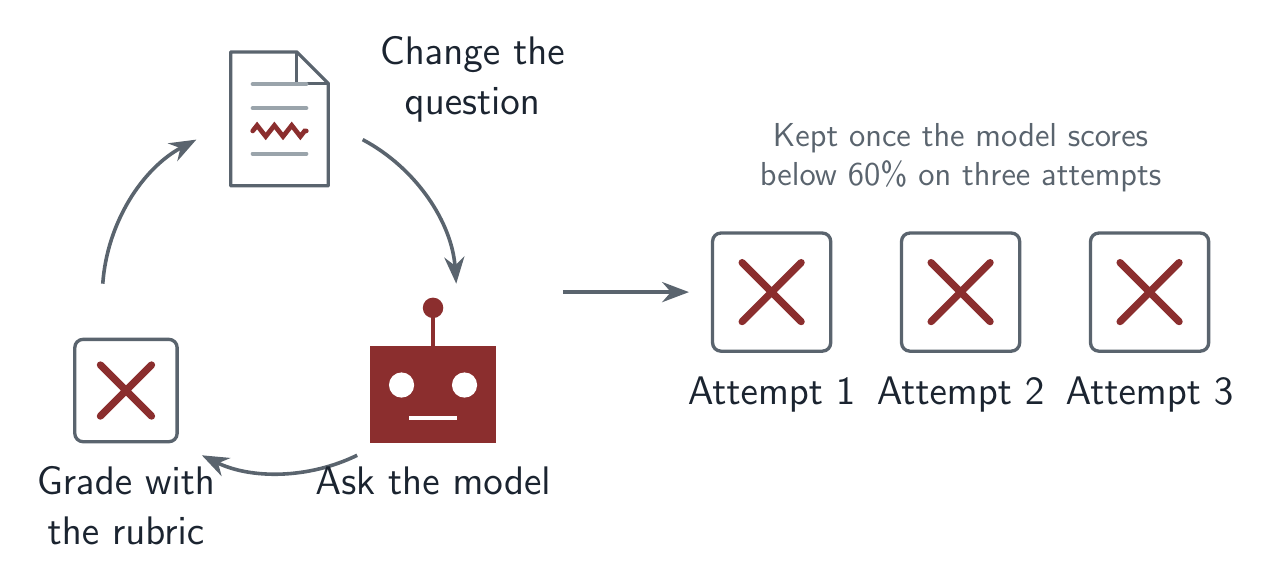
\begin{tikzpicture}[font=\sffamily]
  \begin{scope}[shift={(3.4,3.3)}]
    \def\R{2.25}
    \draw[flow] (62:\R) arc[start angle=62, end angle=4, radius=\R];
    \draw[flow] (-64:\R) arc[start angle=-64, end angle=-116, radius=\R];
    \draw[flow] (176:\R) arc[start angle=176, end angle=118, radius=\R];
    \sheet{-0.62}{1.4}{1.24}{1.7}{red}
    \chatbot{1.95}{-1.25}
    \failcard{-2.6}{-1.85}{1.3}
    \node[lbl, anchor=west] at (1.15,2.75) {Change the\\question};
    \node[lbl, anchor=north] at (1.95,-2.05) {Ask the model};
    \node[lbl, anchor=north] at (-1.95,-2.05) {Grade with\\the rubric};
  \end{scope}
  \draw[flow] (7.0,3.35) -- (8.6,3.35);
  % the test: three attempts, each graded 60% or less
  \foreach \i/\x in {1/8.9,2/11.3,3/13.7} {
    \failcard{\x}{2.6}{1.5}
    \node[lbl, anchor=north] at (\x+0.75,2.4) {Attempt \i};}
  \node[note, anchor=south] at (12.05,4.5) {Kept once the model scores\\below 60\% on three attempts};
\end{tikzpicture}
\end{document}
